\documentclass[11pt, fullpage,letterpaper]{article}

\usepackage[margin=1in]{geometry}
\usepackage{url}
\usepackage{amsmath}
\usepackage{amssymb}
\usepackage{xspace}
\usepackage{graphicx}
\graphicspath{ {./images/} }
\usepackage{hyperref}
\usepackage{listings}


\newcommand{\bx}{{\bf x}}
\newcommand{\bw}{{\bf w}}

\title{CS 6140:Data Mining Project Intemediate-Report}
\author{Ghazal Abdollahi\\ Ajantha Varadharaaj\\ Abdias Baldiviezo}

\begin{document}
\maketitle

% Math commands by Thomas Minka
\newcommand{\var}{{\rm var}}
\newcommand{\Tr}{^{\rm T}}
\newcommand{\vtrans}[2]{{#1}^{(#2)}}
\newcommand{\kron}{\otimes}
\newcommand{\schur}[2]{({#1} | {#2})}
\newcommand{\schurdet}[2]{\left| ({#1} | {#2}) \right|}
\newcommand{\had}{\circ}
\newcommand{\diag}{{\rm diag}}
\newcommand{\invdiag}{\diag^{-1}}
\newcommand{\rank}{{\rm rank}}
% careful: ``null'' is already a latex command
\newcommand{\nullsp}{{\rm null}}
\newcommand{\tr}{{\rm tr}}
\renewcommand{\vec}{{\rm vec}}
\newcommand{\vech}{{\rm vech}}
\renewcommand{\det}[1]{\left| #1 \right|}
\newcommand{\pdet}[1]{\left| #1 \right|_{+}}
\newcommand{\pinv}[1]{#1^{+}}
\newcommand{\erf}{{\rm erf}}
\newcommand{\hypergeom}[2]{{}_{#1}F_{#2}}

% boldface characters
\renewcommand{\a}{{\bf a}}
\renewcommand{\b}{{\bf b}}
\renewcommand{\c}{{\bf c}}
\renewcommand{\d}{{\rm d}}  % for derivatives
\newcommand{\e}{{\bf e}}
\newcommand{\f}{{\bf f}}
\newcommand{\g}{{\bf g}}
\newcommand{\h}{{\bf h}}
%\newcommand{\k}{{\bf k}}
% in Latex2e this must be renewcommand
\renewcommand{\k}{{\bf k}}
\newcommand{\m}{{\bf m}}
\newcommand{\mb}{{\bf m}}
\newcommand{\n}{{\bf n}}
\renewcommand{\o}{{\bf o}}
\newcommand{\p}{{\bf p}}
\newcommand{\q}{{\bf q}}
\renewcommand{\r}{{\bf r}}
\newcommand{\s}{{\bf s}}
\renewcommand{\t}{{\bf t}}
\renewcommand{\u}{{\bf u}}
\renewcommand{\v}{{\bf v}}
\newcommand{\w}{{\bf w}}
\newcommand{\x}{{\bf x}}
\newcommand{\y}{{\bf y}}
\newcommand{\z}{{\bf z}}
%s\newcommand{\l}{\boldsymbol{l}}
\newcommand{\A}{{\bf A}}
\newcommand{\B}{{\bf B}}
\newcommand{\C}{{\bf C}}
\newcommand{\D}{{\bf D}}
\newcommand{\E}{{\bf E}}
\newcommand{\F}{{\bf F}}
\newcommand{\G}{{\bf G}}
\renewcommand{\H}{{\bf H}}
\newcommand{\I}{{\bf I}}
\newcommand{\J}{{\bf J}}
\newcommand{\K}{{\bf K}}
\renewcommand{\L}{{\bf L}}
\newcommand{\M}{{\bf M}}
\newcommand{\N}{\mathcal{N}}  % for normal density
%\newcommand{\N}{{\bf N}}
\renewcommand{\O}{{\bf O}}
\renewcommand{\P}{{\bf P}}
\newcommand{\Q}{{\bf Q}}
\newcommand{\R}{{\bf R}}
\renewcommand{\S}{{\bf S}}
\newcommand{\T}{{\bf T}}
\newcommand{\U}{{\bf U}}
\newcommand{\V}{{\bf V}}
\newcommand{\W}{{\bf W}}
\newcommand{\X}{{\bf X}}
\newcommand{\Y}{{\bf Y}}
\newcommand{\Z}{{\bf Z}}

% this is for latex 2.09
% unfortunately, the result is slanted - use Latex2e instead
%\newcommand{\bfLambda}{\mbox{\boldmath$\Lambda$}}
% this is for Latex2e
\newcommand{\bfLambda}{\boldsymbol{\Lambda}}

% Yuan Qi's boldsymbol
\newcommand{\bsigma}{\boldsymbol{\sigma}}
\newcommand{\balpha}{\boldsymbol{\alpha}}
\newcommand{\bpsi}{\boldsymbol{\psi}}
\newcommand{\bphi}{\boldsymbol{\phi}}
\newcommand{\boldeta}{\boldsymbol{\eta}}
\newcommand{\Beta}{\boldsymbol{\eta}}
\newcommand{\btau}{\boldsymbol{\tau}}
\newcommand{\bvarphi}{\boldsymbol{\varphi}}
\newcommand{\bzeta}{\boldsymbol{\zeta}}

\newcommand{\blambda}{\boldsymbol{\lambda}}
\newcommand{\bLambda}{\mathbf{\Lambda}}
\newcommand{\bOmega}{\mathbf{\Omega}}
\newcommand{\bomega}{\mathbf{\omega}}
\newcommand{\bPi}{\mathbf{\Pi}}

\newcommand{\btheta}{\boldsymbol{\theta}}
\newcommand{\bpi}{\boldsymbol{\pi}}
\newcommand{\bxi}{\boldsymbol{\xi}}
\newcommand{\bSigma}{\boldsymbol{\Sigma}}

\newcommand{\bgamma}{\boldsymbol{\gamma}}
\newcommand{\bGamma}{\mathbf{\Gamma}}

\newcommand{\bmu}{\boldsymbol{\mu}}
\newcommand{\1}{{\bf 1}}
\newcommand{\0}{{\bf 0}}

% \newcommand{\comment}[1]{}

\newcommand{\bs}{\backslash}
\newcommand{\ben}{\begin{enumerate}}
\newcommand{\een}{\end{enumerate}}

 \newcommand{\notS}{{\backslash S}}
 \newcommand{\nots}{{\backslash s}}
 \newcommand{\noti}{{\backslash i}}
 \newcommand{\notj}{{\backslash j}}
 \newcommand{\nott}{\backslash t}
 \newcommand{\notone}{{\backslash 1}}
 \newcommand{\nottp}{\backslash t+1}
% \newcommand{\notz}{\backslash z}

\newcommand{\notk}{{^{\backslash k}}}
%\newcommand{\noti}{{^{\backslash i}}}
\newcommand{\notij}{{^{\backslash i,j}}}
\newcommand{\notg}{{^{\backslash g}}}
\newcommand{\wnoti}{{_{\w}^{\backslash i}}}
\newcommand{\wnotg}{{_{\w}^{\backslash g}}}
\newcommand{\vnotij}{{_{\v}^{\backslash i,j}}}
\newcommand{\vnotg}{{_{\v}^{\backslash g}}}
\newcommand{\half}{\frac{1}{2}}
\newcommand{\msgb}{m_{t \leftarrow t+1}}
\newcommand{\msgf}{m_{t \rightarrow t+1}}
\newcommand{\msgfp}{m_{t-1 \rightarrow t}}

\newcommand{\proj}[1]{{\rm proj}\negmedspace\left[#1\right]}
\newcommand{\argmin}{\operatornamewithlimits{argmin}}
\newcommand{\argmax}{\operatornamewithlimits{argmax}}

\newcommand{\dif}{\mathrm{d}}
\newcommand{\abs}[1]{\lvert#1\rvert}
\newcommand{\norm}[1]{\lVert#1\rVert}

%miscellaneous symbols
\newcommand{\ie}{{{i.e.,}}\xspace}
\newcommand{\eg}{{{\em e.g.,}}\xspace}
\newcommand{\EE}{\mathbb{E}}
\newcommand{\VV}{\mathbb{V}}
\newcommand{\sbr}[1]{\left[#1\right]}
\newcommand{\rbr}[1]{\left(#1\right)}
\newcommand{\cmt}[1]{}





\section{Analyzing Traffic Flow Patterns on AzureFunctionsDataset2019 through Clustering}
\begin{flushleft}
For context refer to our \href{https://docs.google.com/document/d/1YZWRAKUY1-olLNxKiGHXPn6K3Xnj0rWkXE69JiJCMlA/edit?usp=sharing}{(Proposal)}.
and our \href{https://docs.google.com/document/d/1YZWRAKUY1-olLNxKiGHXPn6K3Xnj0rWkXE69JiJCMlA/edit?usp=sharing}{(Data Collection Report)}.\\
 Data can be found in our \href{https://github.com/Azure/AzurePublicDataset}{(Github Repo)} which is a preprocessed version of
\href{https://github.com/Azure/AzurePublicDataset/blob/master/AzureFunctionsDataset2019.md}{(Microsoft's AzurePublicDataset)}.

\end{flushleft}

\section{Progress made towards our goal}
\begin{flushleft}
Our progress can me summarized in the findings that resulted of our collection, pre-processing, processing and
implementation of clustering algorithms to our "Dataset". This application has showed differences in our data points
with which the data can be separated and clustered.
\end{flushleft}

\section{What worked well and what did not?}
\begin{flushleft}
Our team decided to each take some clustering methods and test them with our data.
\begin{enumerate}
    \item \underline{Successes.} Some notable successes in the development of our project were: first, being able to see
    clearer separations between the clusters after dimensionality reduction and second, recolecting different aspects of
    the relationships between datapoints from the implementation and hyperparameter tunning in each of our 5 different clustering methods.

    \item \underline{Challenges.} Using all features that our dataset contains has yielded suboptimal results,
    with a very confusing separation of the data, perhaps because of the low correlations between certain
    features, to mitigate this aspect we used dimensionality reduction in 2 forms: Feature extraction and Feature
    selection. Another challenge we faced was long computational times due to the size of our data (approx. 619368)
    for this we were driven to use a combination of PCA and sub-sampling, which decreased our wait times
    and gave us more freedom in trying different experiments.
\end{enumerate}

\end{flushleft}

\section{What could be done to improve the basic approaches?}
\begin{flushleft}
    Some improvements that were done/considered during development were:
    \begin{itemize}
        \item Using PCA (one or more rounds), tune "n" principal components and variance threshold.
        \item Use HDBSCAN instead of DBSCAN which transforms space according to density/sparsity.
        \item Omitting the sparse points with a very significant Euclidean distance from all of the centroids.
        \item Ommiting mine values, whcih drag the centroids to themselves.
        \item Use libraries that make use of GPUs to achieve faster processing times (CuML).
        \item Using metrics to evaluate clustering performance, for example: Elbow method, ARI, and Silhouette Score (knee point).
    \end{itemize}
\end{flushleft}

\section{Experiments}
\begin{flushleft}
    This is a compact summarization of many steps that went into these experiments.
    \begin{enumerate}
        \item \textbf{K-means, birch, and fuzzy} Preprocessing involved almost all of the items
        in the list above (Fig 1.) which drew the natural shape of the dataset and after normalization (Fig 2-3)
        and another round of PCA revealed a good separation between clusters. The cosine distance
        was also calculated between each pair (Fig 4).
        \break
        \begin{figure}
            \begin{minipage}{0.5\textwidth}
                \caption{Outlier and Mine Omission}
                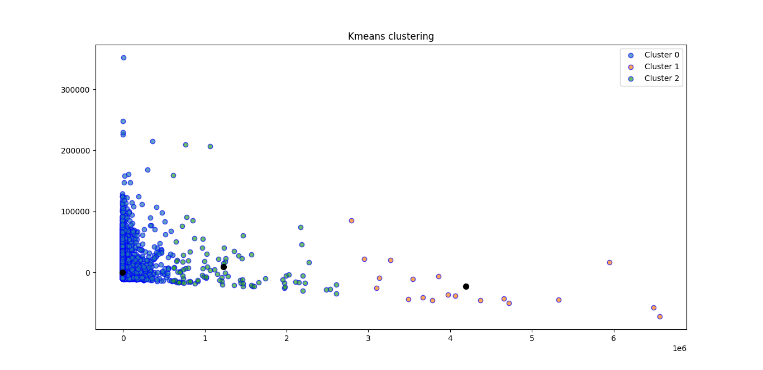
\includegraphics[scale=1.0]{ga1}
            \end{minipage}
            \begin{minipage}{0.5\textwidth}
                \caption{Normalized Data}
                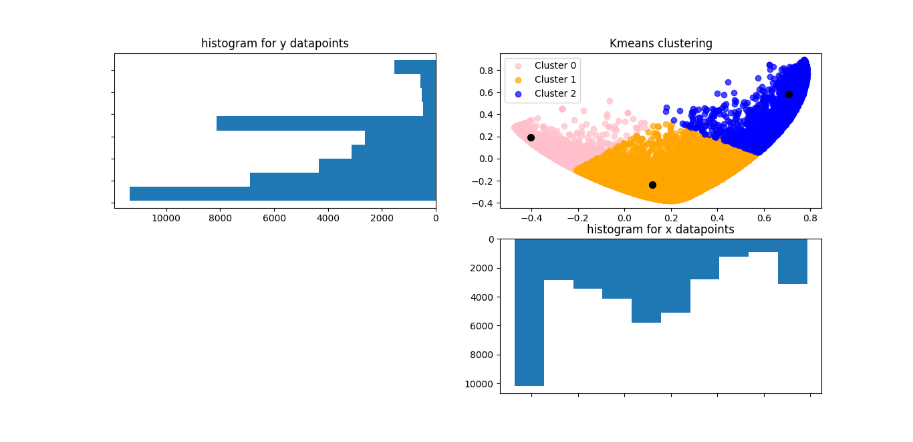
\includegraphics[scale=1.0]{ga2}
            \end{minipage}
            \begin{minipage}{0.5\textwidth}
                \caption{Normalized Data - Heatmap}
                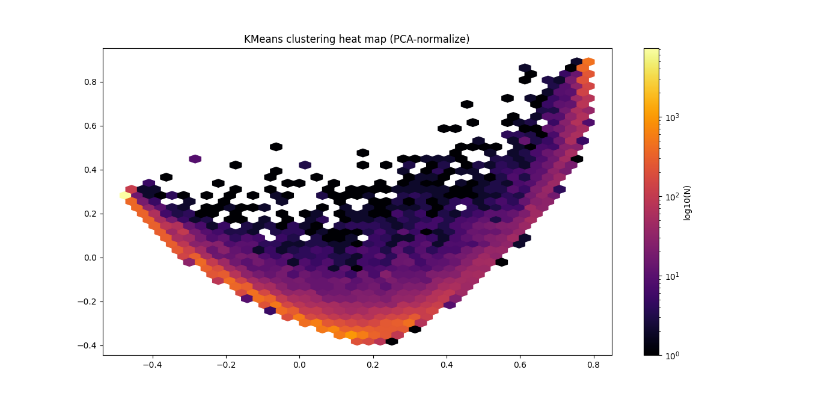
\includegraphics[scale=1.0]{ga3}
            \end{minipage}
            \begin{minipage}{0.5\textwidth}
                \caption{Cosine distance after 4 rounds of PCA}
                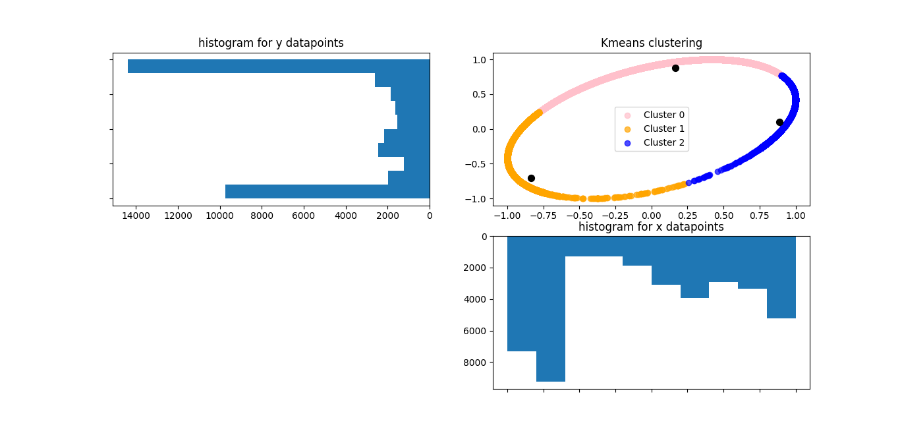
\includegraphics[scale=1.0]{ga4}
            \end{minipage}
        \end{figure}
        \break
        \item \textbf{DBSCAN hyperparameters} Preprocessing to implement DBSCAN was crucial and relied on analysis (Fig 5)
        to find the correct hyperparameters for clustering e.g. Silhouette Score (Fig 6).
        \begin{figure}
            \begin{minipage}{0.5\textwidth}
                \caption{Cumulative variance ratio versus the number of Components}
                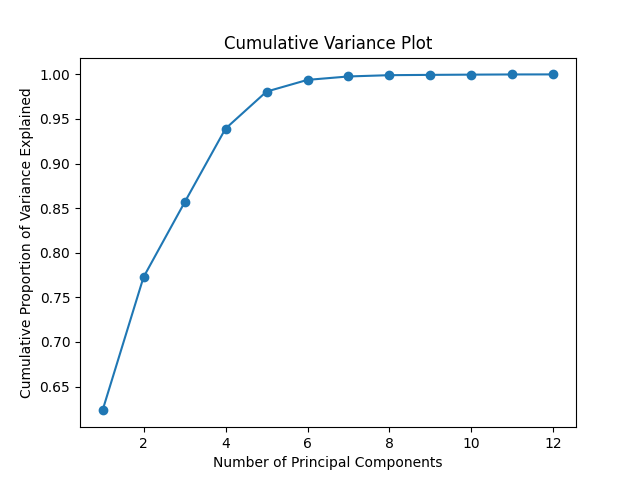
\includegraphics[scale=0.5]{aj1}
            \end{minipage}
            \begin{minipage}{0.5\textwidth}
                \caption{Finding Knee Point}
                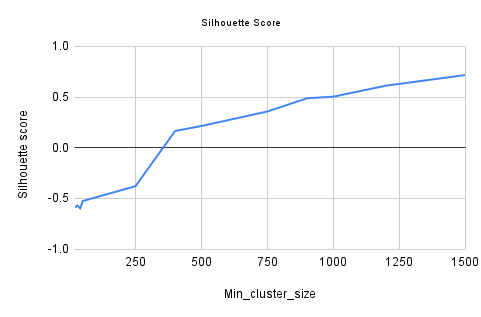
\includegraphics[scale=0.5]{aj2}
            \end{minipage}
        \end{figure}
        \break
        \item \textbf{DBSCAN subsampling} Feature selection was used for dimensionality reduction, as well 
        as subsampling for reasonable computing times. The size of the samples was $20000$ out of $\approx$ $650000$
        datapoints. The features used are "Average", "Count", "Trigger"(Fig 7). 
        Important parameters were eps (\"...maximum distance between two samples for one to be considered as in the neighborhood 
        of the other\") and $min\_samples$ (\"The number of samples or total weight in a neighborhood for 
        a point to be considered as a core point. This includes the point itself.\"), after trying 
        different combinations of these and because of the size of the dataset, the following 
        parameters were the ones that showed more promising results: $eps=0.5$ and $min\_samples=100$.
        \begin{figure}
            \begin{minipage}{0.5\textwidth}
                \caption{Approximate number of clusters using DBSCAN}
                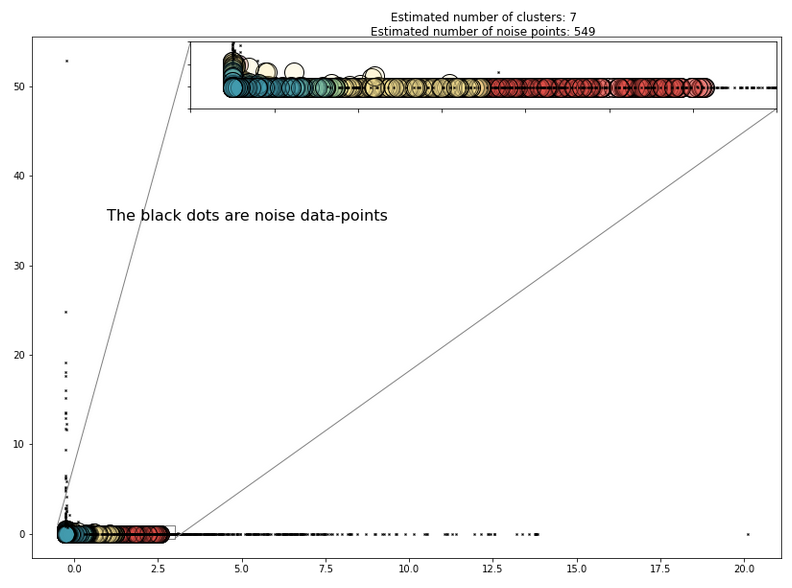
\includegraphics[scale=0.30]{ab1}
            \end{minipage}
            \begin{minipage}{0.5\textwidth}
                \caption{Approximate number of clusters using EM}
                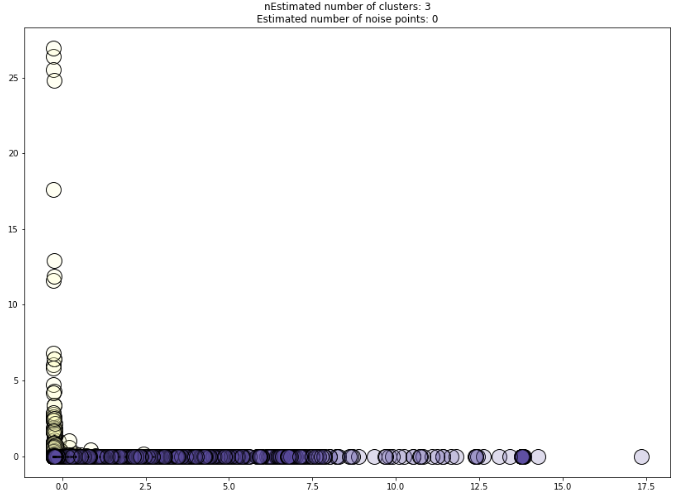
\includegraphics[scale=0.35]{ab2}
            \end{minipage}
        \end{figure}
        \break
        \item \textbf{Expectation maximization clustering (Gaussian Mixture)} The covariance matrix
        and the number of components (The number of mixture components.) were the most important
        parameters in this experiment. The best separation of data was achieved using $n\_components=3$
        and $covariance\_type=diag$ (meaning diagonal).
        Using features ("Average", "Count", "Trigger"), it produced a separation of data
        vertically and horizontally in contrast to DBSCAN (Fig 8).
    \end{enumerate}
\end{flushleft}

\end{document}